\documentclass{tudelftposter}
\usepackage{graphicx}
\usepackage{subfigure}
\title{TI2716-B License plate recognition, Poster 1}

\addauthornote{tu}{Group 2, Delft University of Technology}

\addauthor[tu]{Yinghao Dai}
\addauthor[tu]{Yanna van der Vlugt}

\addfootimage(c:right column.center)[Delft Institute of Applied Mathematics]{tudelft}


\begin{document}
\maketitle
\section{Introduction}
We are working on a license plate recognizer, which can, as the name already suggests, recognize license plates on cars under certain conditions. In the following, we will take you through the steps we have taken so far, and briefly state our plan for next week. 

\section{Character recognition}
Now that we can find a license plate in a given frame, our focus for this week is recognising the characters in the license plate. To do so, we take the following steps:
\begin{itemize}
\item First, we crop the image so that it only contains the license plate
\item We then remove the objects found at the edge of the image, since it often contains the black border of the plate
\item We select the six largest objects left in the frame, since it is likely that these are the characters found on the plate
\item One by one, these objects are fed through a recognition function, which compares the object to each character that can be found on a license plate using the standard Dutch license plate font, and returns the character with which the object differs least
\item The six returned characters are then format-checked, in order to place hyphens in the correct places according to the standard formats for Dutch license plates
\end{itemize}
Shown below is a successful example of this method, where the six characters are located and recognized as "43-JS-RT".

\begin{figure}[h]
	\centering
	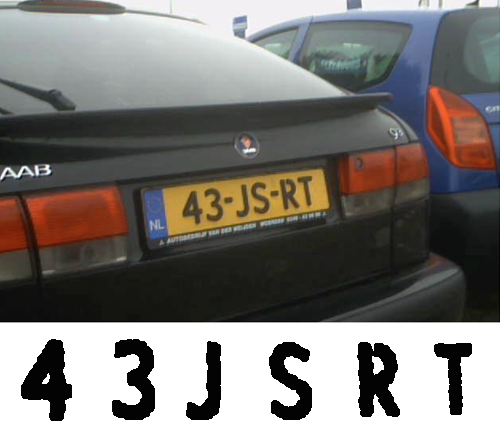
\includegraphics[width=800pt]{goodcar.png}
\end{figure}

\section{Problems}
However, this method does not work ideally for all license plates. We ran into three significant issues:
\begin{itemize}
\item The recognition function often mixed up 'S' with '5' and 'B' with '8'. We were able to solve this issue by giving more weight to the corners of the characters when one of these four was recognised.
\item For some frames, the license plate recognition does not work well yet due to large variations in brightness and white balance. We will focus on standardising the frames to have the same brightness and white balance before thresholding next week.
\item Some characters got split up into two objects during the thresholding process, which resulted in faulty recognition. For example, figure ... shows a license plate where the N is split into two parts, which are recognised as a '1' and 'V' respectively. This also has to do with standardisation and thresholding and will hopefully be resolved next week.
\end{itemize}

\begin{figure}[h]
	\centering
	
\includegraphics[width=800pt]{brokenNplate.png}
	\caption{Faulty recognition where "N" is split into the two separate parts shown}
	\label{brokenN}
\end{figure}

\section{Coupling to front end}
In order to efficiently test how well our system works, we coupled the recognition program to our GUI. For now, this works quite slowly and occasionally gives errors when for example not enough characters are recognised in a frame. This can be sped up by making our code more efficient and processing only selected frames.

\section{Focus for next week}
Next week, we aim to resolve the remaining problems with character recognition by improving the standardisation process, and also speed up the frame processing.

\end{document}
%\experimentalblockright{%
%  SPAM:
%  Nulla malesuada porttitor diam. Donec felis erat, congue non, volutpat at,
%  tincidunt tristique, libero.}